\documentclass[main.tex]{subfiles}
\begin{document}
\chapter{Introduction}
Why this data set?
Why deep learning?
What is the context?

\section{Medical Context}
In 2012 34.490 men and 18.030 women in Germany were diagnosed with an illness corresponding to the ICD-10 code C33-34 \cite{koch2015krebs}. This code describes malignant tumors in the breathable tract more generally summarized as lung cancer. 43499 people died from this illness, which makes it one of the most dangerous types of cancer in Germany. The international comparison shows that other countries too suffer under it's impact \ref{fig:cancInt}.

\begin{figure}[ht]
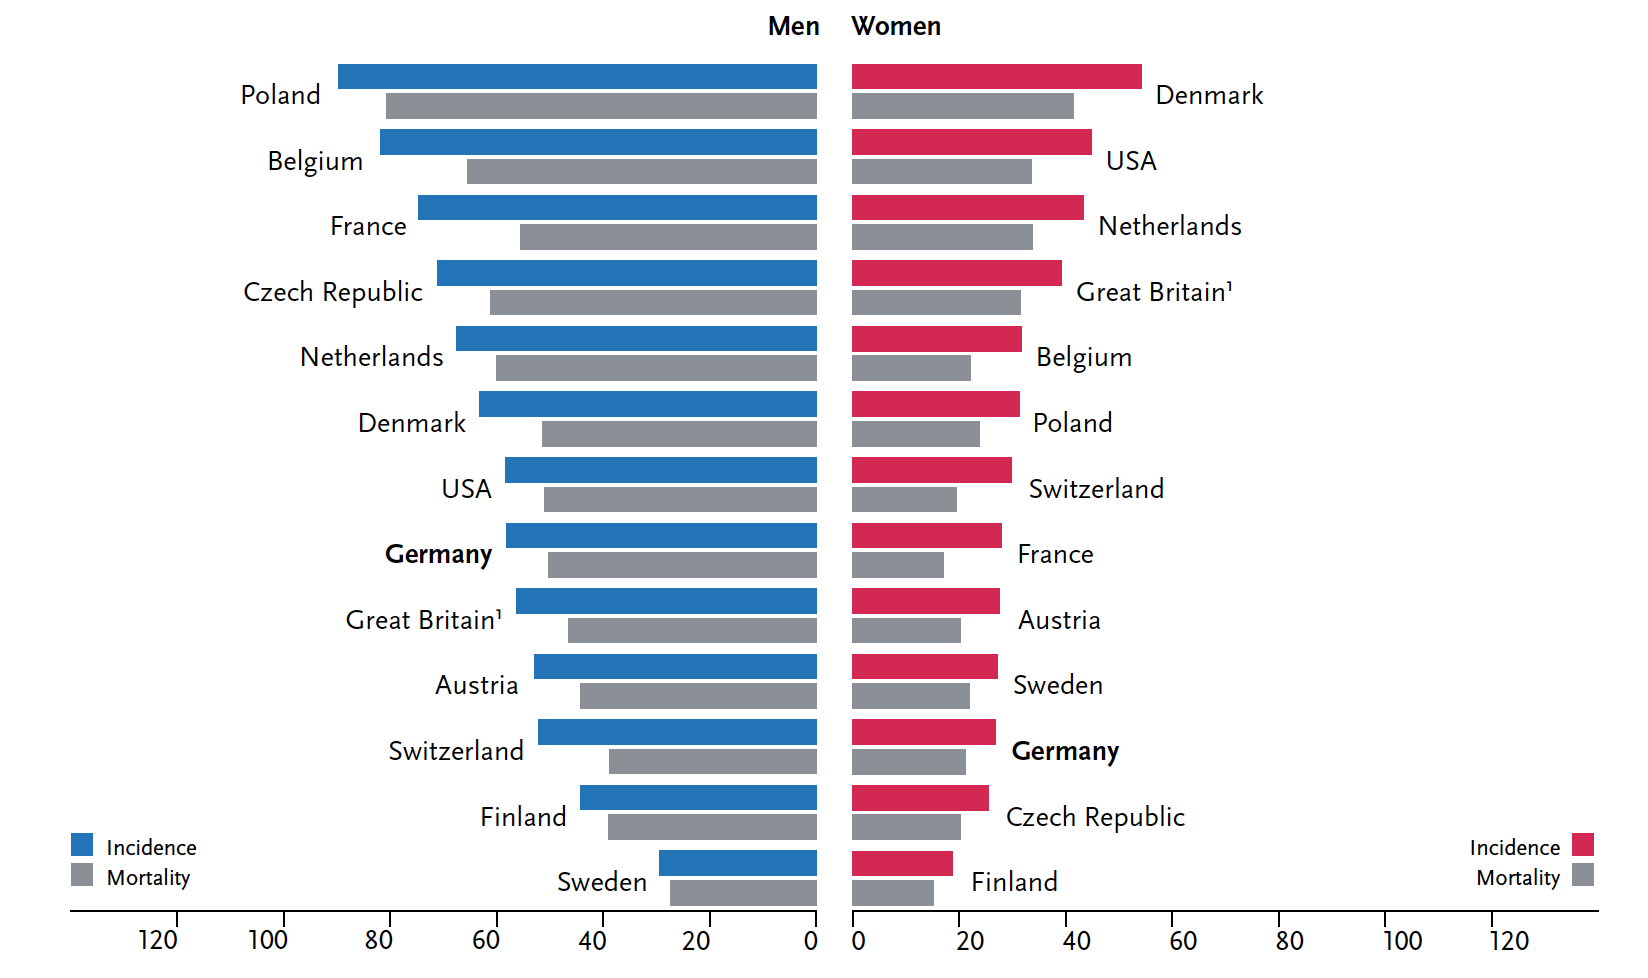
\includegraphics[width=\textwidth]{cancerInternational.png}
\caption{International comparison of age-standardized incidence and mortality rates for lung cancer in the year 2012}
\label{fig:cancInt}
\end{figure}

The main risk factor has been shown to be the exposure to tobacco smoke, whether it's active consumption via cigarettes, or passive exposure especially in closed rooms. CT scanners are used to detect irregular tissue in a patients lung region. These irregularities are grouped under the term \textit{pulmonary nodule}. A pulmonary nodule is a small, round (parenchymal) or worm (juxtapleural) shaped lesion in the lungs. Each lesion has a chance to be malignant and may grow and spread over time, becoming a risk for the patients life in the form of lung cancer. Nodules come not only in different shapes but differ along other features as well. Ground-glass opacity (GGO) nodules are a challenging kind of nodules since they are not thoroughly solid and so harder to detect on a CT scan. The location of the nodules is crucial for the detection rate since nodules close to bigger vessels or the chest wall do not differ much in intensity to the surrounding tissue and can be easily overlooked by the radiologist.


\section{Current Medical Approach}

Patients typically present with fatigue, weight loss, cough, dyspnea, hemoptysis, chest pain
Combination of biopsy and ct scans
Requirement to analyze X pictures per patient
current programs (screenshot OsiriX)
fallacy rates

\section{Opportunities for Assistance}

Early detection of lung cancer is important, because it avoids unnecessary scans in the scenario of undetected cancerous material and it improves the error rate of radiologists.

There exist many algorithmic approaches to finding nodules in CT-Scans \cite{papers_classical} and some that
make use of deep convolutional neural networks to solve related tasks \cite{papers_dnn}\\

Despite much effort being devoted to the computer-aided nodule detection problem, lung CAD systems remain an ongoing
research topic [18]. One of the major difficulties is the detection of GGO nodules with low-dose thin-slice CT screening. Another two difficulties are the detection of nodules that are adjacent to vessels or the chest wall when they have very similar intensity; and the detection of nodules that are nonspherical in shape. In such cases, intensity thresholding or model-based methods might fail to identify those nodules.

\section{Gaining insights from Deep Neural Networks}
Neural networks are strong tools that recently have been shown to solve all kind of problems. They can play
computer games and drive a car, they can create new art and play go to name only a few examples. Yet it seems like the solution they come up with is not intelligible to humans. But in a scenario where medical decisions are based on the output of an algorithm it is crucial that the algorithm is reliable and the way it comes up with a decision is accepted by the people responsible. As long as this is not the case it might still happen that the network produces erroneous results in some cases that did not occur during extensive training.

Strategies to cope with this problem include:
\begin{itemize}
\item Huge databases that contain a variety of samples. In this thesis an open dataset is used that was
the result of a cooperative effort of many scientists and medical staff members and has proven
it's worth in many publications. A possible downside is still that the patients in this database are all Americans and that roughly 1000 patients are not enough to cover all possible cases.

\item Leaving the final decision up to a specialist. This makes sense in many automated processes that decide critical situations. The system is really rather assisting the decision maker. It could compensate a known shortcoming of the human detector or prepare the data in a way that speeds up the process of detection. The further advanced the automated assistance becomes the likelier it gets that the expert might rely too faithfully on it which may be troublesome if the system has build in biases stemming from the distribution of the data.
\end{itemize}

The main issue is that a neural network only remains to be a black box tool as long as no further insights into
the problem can be gained through it's solution. This is why this thesis is concerned with extracting
features and and solution mechanisms from a trained deep neural network on the example of lung CT data. If those extracted features are reasonable for solving the specific problem and they can be conceptualized in terms of already approved procedures, deep neural networks might really aid scientists in understanding novel approaches and solutions.

\end{document}
